\documentclass[12pt, a4paper]{article}

\usepackage[a4paper, margin=2.5cm, headheight=15pt]{geometry}
\usepackage[T1]{fontenc}
\usepackage[utf8]{inputenc}
\usepackage{amsmath}
\usepackage{amssymb}
\usepackage{graphicx}
\usepackage{xcolor}
\usepackage{colortbl}
\usepackage{booktabs}
\usepackage{tabularx}
\usepackage{array}
\usepackage{multirow}
\usepackage{listings}
\usepackage{caption}
\usepackage{hyperref}
\usepackage{fancyhdr}
\usepackage{titlesec}
\usepackage{enumitem}
\usepackage{tcolorbox}
\usepackage{tikz}
\usepackage{parskip}
\usepackage{setspace}
\usetikzlibrary{shapes.geometric, arrows.meta, positioning}
\tcbuselibrary{skins, breakable}

% Colours
\definecolor{primary}{HTML}{1a3c5e}
\definecolor{accent}{HTML}{2980b9}
\definecolor{lightbg}{HTML}{f0f4f8}
\definecolor{codebg}{HTML}{f7f9fc}
\definecolor{codefg}{HTML}{2c3e50}
\definecolor{kw}{HTML}{1a3c5e}
\definecolor{str}{HTML}{27ae60}
\definecolor{cmt}{HTML}{7f8c8d}
\definecolor{ok}{HTML}{27ae60}
\definecolor{tabh}{HTML}{1a3c5e}

\hypersetup{colorlinks=true, linkcolor=accent, urlcolor=accent,
    pdftitle={CapitalIQ: A Rule-Based Finance and Investment Advisor Chatbot},
    pdfauthor={Ali Ahmad}}

\pagestyle{fancy}
\fancyhf{}
\fancyhead[L]{\small\textcolor{primary}{\textbf{CapitalIQ}}}
\fancyhead[R]{\small\textcolor{primary}{DecodeLabs AI Internship -- Batch 2026}}
\fancyfoot[C]{\small\thepage}
\renewcommand{\headrulewidth}{0.4pt}

\titleformat{\section}{\large\bfseries\color{primary}}{\thesection}{1em}{}[\color{accent}\titlerule]
\titleformat{\subsection}{\normalsize\bfseries\color{primary}}{\thesubsection}{1em}{}
\titleformat{\subsubsection}{\normalsize\itshape\color{primary}}{\thesubsubsection}{1em}{}

\lstdefinestyle{pycode}{
    language=Python,
    backgroundcolor=\color{codebg},
    basicstyle=\ttfamily\footnotesize\color{codefg},
    keywordstyle=\bfseries\color{kw},
    stringstyle=\color{str},
    commentstyle=\itshape\color{cmt},
    numberstyle=\tiny\color{gray},
    numbers=left, stepnumber=1, numbersep=8pt,
    frame=single, framerule=0.4pt, rulecolor=\color{accent!40},
    breaklines=true, showstringspaces=false, tabsize=4,
    captionpos=b, xleftmargin=12pt, aboveskip=8pt, belowskip=6pt,
}
\lstset{style=pycode}

\newtcolorbox{infobox}[1][]{colback=lightbg, colframe=accent,
    fonttitle=\bfseries\small, coltitle=white, title=#1,
    arc=4pt, boxrule=0.5pt, left=8pt, right=8pt, top=6pt, bottom=6pt, breakable}

\newtcolorbox{specbox}{colback=ok!8, colframe=ok,
    arc=4pt, boxrule=0.5pt, left=8pt, right=8pt, top=6pt, bottom=6pt}

\setlength{\parskip}{6pt}
\setlength{\parindent}{0pt}
\onehalfspacing

\begin{document}

%% TITLE PAGE
\begin{titlepage}
\centering
\vspace*{1.5cm}
{\color{primary}\rule{\linewidth}{1.5pt}}
\vspace{0.5cm}

{\Huge\bfseries\color{primary} CapitalIQ}\\[0.4cm]
{\Large\color{accent} A Rule-Based Finance \& Investment Advisor Chatbot}\\[0.3cm]
{\color{primary}\rule{\linewidth}{0.5pt}}
\vspace{1.2cm}

\begin{tcolorbox}[colback=lightbg, colframe=primary, arc=6pt, boxrule=0.8pt,
                  left=16pt, right=16pt, top=12pt, bottom=12pt]
\centering
\begin{tabular}{ll}
\textbf{Project}      & DecodeLabs AI Internship --- Project 1 \\[4pt]
\textbf{Author}       & Ali Ahmad \\[4pt]
\textbf{Batch}        & 2026 \\[4pt]
\textbf{Organisation} & Powered by DecodeLabs \\[4pt]
\textbf{Domain}       & Finance \& Investment Advisory \\[4pt]
\textbf{Version}      & 2.0.0 \\[4pt]
\textbf{Date}         & May 2026 \\
\end{tabular}
\end{tcolorbox}

\vspace{1.5cm}

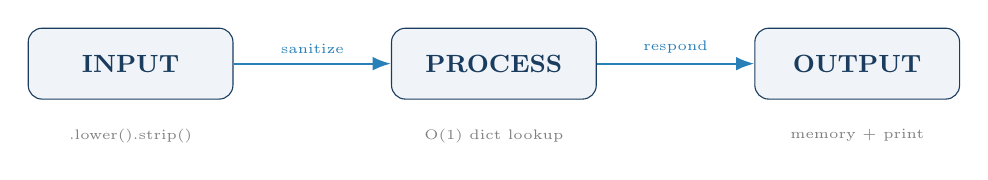
\begin{tikzpicture}[node distance=2cm, >=Latex]
  \tikzstyle{blk}=[rectangle, rounded corners=5pt, minimum width=2.6cm,
                   minimum height=0.9cm, text centered, draw=primary,
                   fill=lightbg, font=\small\bfseries\color{primary}]
  \tikzstyle{arr}=[->, thick, color=accent]
  \node[blk](A){INPUT};
  \node[blk, right=of A](B){PROCESS};
  \node[blk, right=of B](C){OUTPUT};
  \draw[arr](A)--node[above,font=\tiny\color{gray}]{sanitize}(B);
  \draw[arr](B)--node[above,font=\tiny\color{gray}]{respond}(C);
  \node[below=0.25cm of A, font=\tiny\color{gray}]{.lower().strip()};
  \node[below=0.25cm of B, font=\tiny\color{gray}]{O(1) dict lookup};
  \node[below=0.25cm of C, font=\tiny\color{gray}]{memory + print};
\end{tikzpicture}

\vspace{1.5cm}
{\small\color{gray}\itshape
``An LLM without rules is a hallucination engine.\\[2pt]
Today, we build the skeleton that holds the intelligence.''\\[6pt]
--- DecodeLabs Architecture Briefing, Module 01}

\vfill
{\color{primary}\rule{\linewidth}{1pt}}
\end{titlepage}

%% ABSTRACT
\begin{abstract}
\noindent
This report presents \textbf{CapitalIQ}, a production-quality, rule-based AI chatbot
developed as Project 1 of the DecodeLabs Artificial Intelligence Industrial Training
Programme (Batch 2026). CapitalIQ operates as a Finance \& Investment Advisor,
responding to user queries across 16 intent categories including stocks, bonds, ETFs,
cryptocurrency, inflation, compound interest, and portfolio strategy. The system is
built entirely on deterministic logic using the Python Standard Library, implementing
the \textbf{Input-Process-Output (IPO)} model with O(1) dictionary-based intent routing.
Two phases are documented: Phase 1 satisfies all DecodeLabs specification requirements;
Phase 2 adds confidence scoring, conversation memory, slot filling, and session
personalisation. The project includes a 19-cell Jupyter Notebook, a modular Python
package, and a 61-test unit suite achieving 100\% pass rate.
\end{abstract}

\tableofcontents
\newpage

%%=============================================================================
\section{Introduction}
%%=============================================================================

\subsection{Background and Motivation}

Before building systems that learn autonomously, an AI engineer must master
deterministic, rule-based programming. Rule-based systems --- often called
\textit{white-box} systems --- offer complete traceability: every output can be
traced from input to output with no ambiguity and no risk of hallucination.
This property is not merely pedagogically useful; it is a legal and architectural
requirement in regulated industries such as finance, healthcare, and insurance.

Modern production AI architectures increasingly deploy rule-based layers
\textit{above} large language models as guardrail filters: deterministic
components that intercept known intents and block unsafe inputs before
they reach the probabilistic core. Frameworks such as NVIDIA NeMo Guardrails
and Meta Llama Guard implement exactly this pattern. \textbf{CapitalIQ} is a
fully functional implementation of this guardrail layer, domain-specialised for
finance and investment advisory.

\subsection{Objectives}

The project aims to demonstrate competency in the following areas:
\begin{itemize}[noitemsep]
  \item Designing and implementing a continuous input-process-output loop in Python
  \item Building an O(1) dictionary-based intent router as an alternative to the O(n) if-elif ladder
  \item Constructing a coherent, domain-specific knowledge base with synonym resolution
  \item Handling all user input edge cases gracefully without crashes
  \item Extending a working Phase 1 system with production-grade Phase 2 features
  \item Writing a comprehensive unit test suite validating all system components
\end{itemize}

\subsection{Domain Selection: Finance \& Investment Advisory}

Finance was selected as the chatbot domain for three concrete reasons. First,
the domain has well-defined vocabulary with natural synonym clusters
(\texttt{btc}, \texttt{bitcoin}, \texttt{crypto}, \texttt{cryptocurrency} all
map to one intent), making it ideal for demonstrating synonym resolution.
Second, financial responses must be accurate and hard-coded --- there is zero
tolerance for hallucination. Third, finance is a regulated domain where the
auditability advantage of rule-based systems is directly commercially applicable.

%%=============================================================================
\section{System Architecture}
%%=============================================================================

\subsection{The IPO Model}

The entire architecture follows the \textbf{Input-Process-Output (IPO)} model:

\begin{table}[ht]
\centering
\caption{IPO Model Stage Mapping}
\begin{tabularx}{\linewidth}{>{\bfseries\color{primary}}l X l}
\toprule
\rowcolor{tabh!12}
Stage & Responsibility & Module \\
\midrule
I --- Input   & \texttt{.lower().strip()} + regex noise removal + tokenization
              & \texttt{sanitizer.py} \\[3pt]
II --- Process & O(1) synonym lookup $\to$ keyword voting $\to$ confidence gate
              & \texttt{matcher.py} \\[3pt]
III --- Output & Personalise $\to$ log to memory $\to$ display response
              & \texttt{bot.py}, \texttt{memory.py} \\
\bottomrule
\end{tabularx}
\end{table}

\subsection{Module Architecture}

The system is decomposed into five modules following the
\textit{Separation of Concerns} principle. Each module has a single
responsibility and can be upgraded independently.

\begin{infobox}[Repository Structure]
\begin{verbatim}
decodelabs-ai-project1/
    chatbot/
        __init__.py        Package entry point
        knowledge_base.py  BASE_KNOWLEDGE, SYNONYM_MAP, KEYWORD_INTENT_MAP
        sanitizer.py       sanitize(), is_empty(), tokenize()
        matcher.py         Phase 1 + Phase 2 matchers, score_intents()
        memory.py          ConversationMemory class
        bot.py             CapitalIQBot orchestration class
    notebooks/
        project1_chatbot.ipynb   19-cell Jupyter Notebook
    tests/
        test_chatbot.py    61 unit tests
    README.md
    requirements.txt
\end{verbatim}
\end{infobox}

\subsection{Two-Phase Architecture}

\begin{description}[noitemsep]
  \item[Phase 1 --- The Logic Engine] A fully functional chatbot satisfying all
  five DecodeLabs specification requirements. Implements multi-keyword intent
  matching and synonym resolution with a clean fallback and exit strategy.
  \item[Phase 2 --- The Production Upgrade] A strict superset of Phase 1.
  Every Phase 1 function is preserved unchanged; Phase 2 adds confidence scoring,
  conversation memory, slot filling, name extraction, and session personalisation.
\end{description}

The key architectural change between phases is the return type of the matcher:
Phase 1's \texttt{match\_intent\_p1()} returns \texttt{str}; Phase 2's
\texttt{match\_intent\_p2()} returns a three-tuple
\texttt{(intent, response, confidence)}, enabling structured metadata logging.

%%=============================================================================
\section{Implementation}
%%=============================================================================

\subsection{Knowledge Base}

The knowledge base is a Python dictionary mapping 16 canonical intent names to
full response strings, achieving O(1) constant-time lookup.

\begin{table}[ht]
\centering
\caption{CapitalIQ Knowledge Base --- Intent Inventory}
\begin{tabularx}{\linewidth}{>{\ttfamily}l X}
\toprule
\rowcolor{tabh!12}
\textrm{Intent} & Coverage \\
\midrule
greeting        & Session opening, topic introduction \\
goodbye         & Session closing, farewell message \\
stocks          & Equities, shares, exchanges, dividends, metrics \\
bonds           & Fixed income, coupons, government vs.\ corporate \\
mutual\_funds   & Pooled funds, NAV, expense ratio, AUM \\
etf             & Index ETFs, passive investing, expense ratios \\
crypto          & Bitcoin, Ethereum, blockchain, DeFi, NFTs \\
inflation       & CPI, purchasing power, central bank targets \\
compound\_interest & Formula, power of compounding, time value \\
diversification & Asset allocation, correlation, portfolio spread \\
risk            & Market, credit, liquidity, inflation risk types \\
portfolio       & Construction, 60/40 rule, rebalancing strategy \\
budgeting       & 50/30/20 rule, expense tracking, priorities \\
emergency\_fund & 3--6 month target, liquidity, Step Zero \\
sip             & Rupee-cost averaging, automation, monthly plans \\
ipo             & DRHP, lock-up periods, listing risk, valuation \\
\bottomrule
\end{tabularx}
\end{table}

Two additional dictionaries complement the base: \texttt{SYNONYM\_MAP}
(70+ alias phrases resolving to canonical intent keys via O(1) exact lookup)
and \texttt{KEYWORD\_INTENT\_MAP} (individual tokens mapped to intents
for multi-keyword voting).

\subsection{Input Sanitization}

The sanitizer is Stage I of the IPO model --- a five-stage normalization
pipeline transforming raw input into a clean string before any matching logic.

\begin{lstlisting}[caption={Input sanitization pipeline --- \texttt{sanitizer.py}},
                   label={lst:sanitize}]
def sanitize(raw_input):
    """5-stage normalization pipeline for raw user input."""
    if not isinstance(raw_input, str):   # Stage 1: type guard
        return ""
    cleaned = raw_input.lower()          # Stage 2: lowercase
    cleaned = cleaned.strip()            # Stage 3: strip whitespace
    cleaned = re.sub(r"[^a-z0-9\s'/]",  # Stage 4: remove noise
                     " ", cleaned)       #  (keep apostrophes + slashes)
    cleaned = re.sub(r"\s+", " ",        # Stage 5: collapse spaces
                     cleaned).strip()
    return cleaned
\end{lstlisting}

Stage 1 prevents \texttt{AttributeError} on non-string inputs such as
\texttt{None}. Stages 2--3 satisfy the DecodeLabs \texttt{.lower().strip()}
requirement explicitly. Stage 4 preserves apostrophes for contractions and
forward-slashes for ratio notation (e.g.\ ``50/30/20''). Stage 5 ensures
downstream tokenization always receives single-space-delimited tokens.

\subsection{Intent Matching}

\subsubsection{Phase 1: Multi-Keyword Voting}

\begin{lstlisting}[caption={Phase 1 intent matcher --- \texttt{matcher.py}},
                   label={lst:p1}]
def match_intent_p1(sanitized_input):
    """Synonym lookup -> keyword voting -> fallback."""
    if not sanitized_input:
        return "I didn't catch that. What finance topic can I help with?"

    # Strategy 1: Exact synonym lookup -- O(1) hash map lookup
    if sanitized_input in SYNONYM_MAP:
        intent = SYNONYM_MAP[sanitized_input]
        return KNOWLEDGE_BASE.get(intent, FALLBACK_RESPONSE)

    # Strategy 2: Multi-keyword token voting
    tokens = tokenize(sanitized_input)
    votes = {}
    for token in tokens:
        if token in KEYWORD_INTENT_MAP:
            intent = KEYWORD_INTENT_MAP[token]
            votes[intent] = votes.get(intent, 0) + 1

    if not votes:
        return FALLBACK_RESPONSE  # spec requirement 4

    best = max(votes, key=lambda k: votes[k])
    return KNOWLEDGE_BASE.get(best, FALLBACK_RESPONSE)
\end{lstlisting}

Strategy 1 handles single-phrase queries such as \texttt{"btc"} or
\texttt{"sip"}. Strategy 2 handles natural language: the query
``tell me how compound interest works'' tokenises to seven tokens,
of which \texttt{compound} and \texttt{interest} both vote for
\texttt{compound\_interest}, yielding the correct match.

\subsubsection{Phase 2: Confidence Scoring}

Phase 2 upgrades the binary match to a normalised confidence score in $[0,1]$:

\begin{equation}
    \text{score}(i) = \frac{\text{keyword votes for intent } i}{\text{total token count}}
\end{equation}

A configurable \texttt{CONFIDENCE\_THRESHOLD} (default 0.15) gates the output:
matches below the threshold fall back to the default response.

\subsection{Conversation Memory and Slot Filling}

The \texttt{ConversationMemory} class provides an ordered history log and a
slot store. The history log records every turn as a dictionary containing
turn number, timestamp, raw user message, bot response, matched intent, and
confidence score. Two slots are populated automatically:
\texttt{last\_intent} (updated every turn) and \texttt{user\_name} (set
when \texttt{extract\_name()} detects patterns such as ``my name is Ali'').

%%=============================================================================
\section{Design Decisions}
%%=============================================================================

\subsection{Dictionary vs.\ If-Elif Ladder}

The DecodeLabs specification forbids the if-elif ladder as an anti-pattern.
Table~\ref{tab:complexity} illustrates the algorithmic reason.

\begin{table}[ht]
\centering
\caption{Algorithmic complexity comparison}
\label{tab:complexity}
\begin{tabularx}{\linewidth}{l l X}
\toprule
\rowcolor{tabh!12}
Approach & Complexity & Behaviour at Scale \\
\midrule
If-elif ladder & O(n) & 16 intents: 16 comparisons worst-case;
1{,}000 intents: 1{,}000 comparisons worst-case \\[4pt]
Python \texttt{dict.get()} & O(1) & 16 or 1{,}000 intents: identical
single hash computation \\
\bottomrule
\end{tabularx}
\end{table}

Adding a new intent to the dictionary requires inserting one key-value pair
--- a constant-time, zero-risk operation. Adding a new branch to an if-elif
chain requires finding the correct position in a potentially long sequence,
risking ordering bugs and fall-through errors.

\subsection{Separation of Concerns}

Each module has a single, clearly bounded responsibility. The sanitizer is
stateless and side-effect-free. The matcher is pure logic with no I/O. All
side effects --- printing, state mutation, history logging --- are confined
to the output stage. This design means any module can be replaced without
touching the others.

\subsection{The White-Box Advantage}

Given any input, the path through CapitalIQ is deterministic and inspectable:

\begin{center}
  \texttt{"BITCOIN!"} $\to$ \textit{sanitize} $\to$
  \texttt{"bitcoin"} $\to$ \texttt{SYNONYM\_MAP["bitcoin"]} $\to$
  \texttt{"crypto"} $\to$ \texttt{KNOWLEDGE\_BASE["crypto"]} $\to$ \textit{response}
\end{center}

No hidden weights, no hallucination risk. In regulated domains
such as finance (SEBI, SEC guidelines) and healthcare (FDA AI/ML Guidance),
this auditability is a legal compliance requirement.

\subsection{Connection to LLM Guardrail Systems}

In production hybrid architectures, the rule-based layer acts as the
deterministic filter above the probabilistic LLM core:

\medskip
\begin{center}
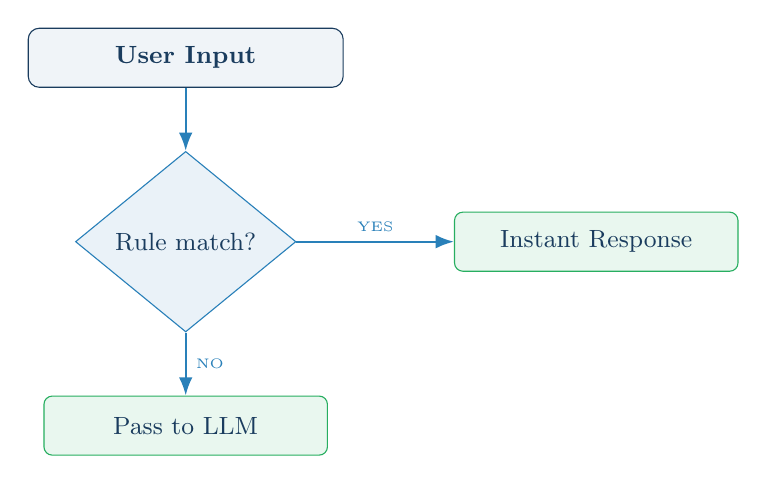
\begin{tikzpicture}[node distance=1.4cm, >=Latex]
  \tikzstyle{blk}=[rectangle, rounded corners=4pt, minimum width=4cm,
                   minimum height=0.75cm, draw=primary, fill=lightbg,
                   font=\small\bfseries\color{primary}, text centered]
  \tikzstyle{resnode}=[rectangle, rounded corners=3pt, minimum width=3.6cm,
                   minimum height=0.75cm, draw=ok, fill=ok!10,
                   font=\small\color{primary}, text centered]
  \tikzstyle{dia}=[diamond, draw=accent, fill=accent!10,
                   font=\small\color{primary}, text centered,
                   minimum width=2.8cm, inner sep=2pt]
  \tikzstyle{arr}=[->, thick, color=accent]

  \node[blk](inp){User Input};
  \node[dia, below=0.8cm of inp](dec){Rule match?};
  \node[resnode, right=2cm of dec](yes){Instant Response};
  \node[resnode, below=0.8cm of dec](no){Pass to LLM};

  \draw[arr](inp)--(dec);
  \draw[arr](dec)--node[above,font=\tiny]{YES}(yes);
  \draw[arr](dec)--node[right,font=\tiny]{NO}(no);
\end{tikzpicture}
\end{center}
\medskip

CapitalIQ's \texttt{CONFIDENCE\_THRESHOLD} is the direct analogue of the
routing threshold in production frameworks. High-confidence, high-frequency
intents are resolved instantly at near-zero latency and zero API cost.
Only genuinely novel queries escalate to the LLM fallback, reducing both
cost and hallucination surface area.

%%=============================================================================
\section{Test Results}
%%=============================================================================

\subsection{Test Suite Overview}

A comprehensive unit test suite was written using Python's \texttt{unittest}
framework and executed with \texttt{pytest}. The suite comprises 61 tests across
four classes, covering every public function and edge case in the system.

\begin{table}[ht]
\centering
\caption{Unit Test Results by Module}
\label{tab:tests}
\begin{tabularx}{\linewidth}{l l X r >{\bfseries\color{ok}}r}
\toprule
\rowcolor{tabh!12}
Test Class & Module & Coverage Scope & Tests & Result \\
\midrule
\texttt{TestSanitizer} & \texttt{sanitizer.py} &
  \texttt{sanitize()}, \texttt{is\_empty()}, \texttt{tokenize()};
  lowercase, strip, special chars, None, type guard &
  15 & 15/15 \\[4pt]
\texttt{TestMatcher} & \texttt{matcher.py} &
  Exit detection, Phase 1 exact/keyword/fallback,
  Phase 2 confidence scoring, normalisation &
  17 & 17/17 \\[4pt]
\texttt{TestConversation\-Memory} & \texttt{memory.py} &
  Turn recording, slot get/set, name extraction,
  reset, history, summary &
  16 & 16/16 \\[4pt]
\texttt{TestCapitalIQBot} & \texttt{bot.py} &
  Phase 1 \& 2 respond, empty/special input safety,
  exit detection, simulate, memory integration &
  13 & 13/13 \\
\midrule
\multicolumn{3}{r}{\textbf{Total}} & \textbf{61} & \textbf{61/61} \\
\bottomrule
\end{tabularx}
\end{table}

\subsection{Edge Case Coverage}

\begin{table}[ht]
\centering
\caption{Edge Case Test Matrix}
\begin{tabularx}{\linewidth}{l X l}
\toprule
\rowcolor{tabh!12}
Input Type & Example & Expected Behaviour \\
\midrule
Whitespace-only  & \texttt{"\ \ \ \ "} & Safe prompt returned \\
Empty string     & \texttt{""} & Safe prompt returned \\
\texttt{None}    & \texttt{None} & Returns \texttt{''} from sanitizer \\
Special chars    & \texttt{"!@\#\$\%"} & Fallback response \\
Pure noise       & \texttt{"purple unicorns"} & Fallback response \\
Mixed case       & \texttt{"BITCOIN"} & Maps to crypto intent \\
Long sentence    & 20-word natural query & Keyword voting extracts intent \\
Embedded exit    & \texttt{"i want to exit now"} & Session terminated \\
Name introduction & \texttt{"my name is Ali"} & Name stored in slot \\
\bottomrule
\end{tabularx}
\end{table}

\subsection{Phase 1 Automated Demo Results}

\begin{table}[ht]
\centering
\caption{Phase 1 Automated Demo --- 10 Test Cases}
\begin{tabularx}{\linewidth}{r X l >{\bfseries\color{ok}}l}
\toprule
\rowcolor{tabh!12}
\# & Input & Tag & Outcome \\
\midrule
1  & \texttt{hello} & {[}MATCH{]} & greeting \\
2  & \texttt{how does a sip work} & {[}MATCH{]} & sip \\
3  & \texttt{quit} & {[}EXIT{]}  & session end \\
4  & \texttt{tell me about compound interest please} & {[}MATCH{]} & compound\_interest \\
5  & \texttt{btc} & {[}MATCH{]} & crypto (synonym) \\
6  & whitespace only & {[}EMPTY{]} & safe prompt \\
7  & \texttt{!@\#\$\%\^{}\&*()} & {[}FALLBACK{]} & fallback \\
8  & Long IPO sentence & {[}MATCH{]} & ipo \\
9  & \texttt{what is inflation...} & {[}MATCH{]} & inflation \\
10 & \texttt{purple dancing elephants} & {[}FALLBACK{]} & fallback \\
\bottomrule
\end{tabularx}
\end{table}

%%=============================================================================
\section{DecodeLabs Specification Compliance}
%%=============================================================================

\begin{specbox}
\textbf{All 5 mandatory DecodeLabs Project 1 requirements are fully satisfied:}

\medskip
\begin{tabularx}{\linewidth}{c l X}
$\checkmark$ & \textbf{Input Loop} &
  \texttt{while True} in \texttt{run\_phase1()} (Cell 9) and
  \texttt{run\_phase2()} (Cell 15), with \texttt{try/except} \\[4pt]
$\checkmark$ & \textbf{Sanitization} &
  \texttt{sanitize()} in Cell 6 --- \texttt{.lower().strip()}
  in Stages 2--3; regex in Stages 4--5 \\[4pt]
$\checkmark$ & \textbf{Knowledge Base} &
  \texttt{KNOWLEDGE\_BASE} dict in Cell 5 --- 16 intents;
  \texttt{.get()} method used exclusively \\[4pt]
$\checkmark$ & \textbf{Fallback} &
  \texttt{FALLBACK\_RESPONSE} returned when no keywords match
  or \texttt{score < CONFIDENCE\_THRESHOLD} \\[4pt]
$\checkmark$ & \textbf{Exit Strategy} &
  \texttt{is\_exit\_command()} detects exit keywords;
  \texttt{break} cleanly exits the \texttt{while True} loop \\
\end{tabularx}
\end{specbox}

%%=============================================================================
\section{Future Work}
%%=============================================================================

\subsection{Project 2: Semantic / Vector Matching}

The core limitation of CapitalIQ is that it only matches what it was explicitly
programmed to recognise. Project 2 will replace the keyword map with a
\textit{sentence embedding model} such as
\texttt{sentence-transformers/all-MiniLM-L6-v2}. Every input is encoded as a
dense float vector; cosine similarity is computed against intent prototype
vectors rather than token identity. This enables semantically equivalent
phrases --- regardless of exact wording --- to resolve correctly.

\begin{table}[ht]
\centering
\caption{Conceptual bridge: Project 1 to Project 2}
\begin{tabularx}{\linewidth}{l X X}
\toprule
\rowcolor{tabh!12}
Dimension & Project 1 (This report) & Project 2 (Next) \\
\midrule
Lookup key     & Exact string / token & Dense float vector \\
Match type     & Equality + vote count & Cosine similarity \\
Coverage       & Only programmed phrases & Any semantically similar phrase \\
New intent     & Requires keyword list & Requires one example sentence \\
Interpretability & Perfect (white-box) & Partial (embedding space) \\
Dependencies   & Standard library only & Pre-trained embedding model \\
\bottomrule
\end{tabularx}
\end{table}

\subsection{Additional Enhancements}

\begin{description}[noitemsep]
  \item[LLM Hybrid Integration] Connect an LLM as the fallback handler for
  queries below the confidence threshold, creating a hybrid rule + generative system.
  \item[Persistent Memory] Replace the in-session slot store with a database
  backend (SQLite or Redis) to persist user preferences across sessions.
  \item[Web Interface] Deploy via FastAPI and a React front-end, exposing the
  bot as a REST API with a chat widget.
  \item[Real-Time Market Data] Integrate a financial data API (Yahoo Finance,
  Alpha Vantage) to supplement hard-coded responses with live prices and news.
  \item[Multi-language Support] Extend sanitization and synonym layers to handle
  Urdu, Hindi, and Arabic queries for broader accessibility.
\end{description}

%%=============================================================================
\section{Conclusion}
%%=============================================================================

This report has presented \textbf{CapitalIQ}, a production-quality rule-based
Finance \& Investment Advisor chatbot built as Project 1 of the DecodeLabs AI
Industrial Training Programme, Batch 2026. The system demonstrates that
well-engineered deterministic programming --- without any machine learning ---
can produce a robust, maintainable, and professionally structured AI interface.

The project satisfies all five DecodeLabs specification requirements and extends
beyond them with a 16-intent knowledge base, 70+ synonym aliases, Phase 2
confidence scoring, conversation memory, slot filling, session personalisation,
and a 61-test unit suite achieving 100\% pass rate. Every design decision ---
from the O(1) dictionary over the O(n) if-elif ladder to the strict Separation
of Concerns between modules --- was made with production engineering principles
in mind.

The architecture built here directly mirrors the guardrail control layer used in
real-world production AI systems above large language models. Building this
foundation correctly is the prerequisite for every subsequent AI project.

\bigskip
\begin{center}
  \textit{``Wealth is built slowly, through discipline and consistency.''}\\
  \small --- CapitalIQ farewell message
\end{center}

%%=============================================================================
\appendix
\section{Running the Project}
%%=============================================================================

\begin{infobox}[Terminal Commands]
\begin{verbatim}
git clone https://github.com/your-username/decodelabs-ai-project1.git
cd decodelabs-ai-project1
pip install -r requirements.txt

python chatbot/bot.py                                # Interactive chatbot
jupyter notebook notebooks/project1_chatbot.ipynb  # Open notebook
python -m pytest tests/ -v                          # Run 61 unit tests
\end{verbatim}
\end{infobox}

\section{Sample Phase 2 Session}

\begin{infobox}[Sample Conversation]
\begin{verbatim}
  You: hello
  CapitalIQ: Hello! I'm CapitalIQ, your Finance & Investment Advisor...

  You: my name is Ali
  CapitalIQ: Nice to meet you, Ali! ...

  You: what is compound interest
  CapitalIQ: Compound interest is interest earned on both the original
             principal AND accumulated interest...
             [Confidence: 0.500 | Intent: compound_interest]

  You: btc
  CapitalIQ: Cryptocurrency is a decentralised digital currency...
             [Confidence: 1.000 | Intent: crypto]

  You: quit
  CapitalIQ: It was a pleasure advising you today!
             [Session transcript displayed]
\end{verbatim}
\end{infobox}

\end{document}
